\documentclass[12pt]{article}
\usepackage{times}
\usepackage[english]{babel}
\usepackage[utf8x]{inputenc}
\usepackage[colorinlistoftodos]{todonotes}
\usepackage[margin=1in]{geometry}
\usepackage{graphicx}
\usepackage{subcaption}
\usepackage{epstopdf}
\usepackage{cite}
\usepackage{listings}
\usepackage{dtklogos}
\usepackage{wrapfig}
\usepackage{amsmath}
\usepackage{amsthm}
\usepackage{amssymb}
\usepackage{amscd}
\usepackage{caption}
\usepackage{etoolbox}
\usepackage{fancyhdr}
\usepackage{stackengine}
\usepackage[export]{adjustbox}
\patchcmd{\thebibliography}{\section*{\refname}}{}{}{}
\usepackage[document]{ragged2e}    %This causes text to left align
\usepackage[colorlinks=true, linkcolor=black,citecolor=black,urlcolor=blue]{hyperref}
\bibliographystyle{IEEEtran}
\DeclareGraphicsRule{.tif}{png}{.png}{`convert #1 `dirname #1`/`basename #1 .tif`.png}

\title{MCHE 220: Report 3}

\begin{document}
\lefthyphenmin3
\righthyphenmin4
% \pretolerance=2000
% \tolerance=500 
% \emergencystretch=10pt
\raggedright     %Stops LaTeX from automatically hyphenating the right margin to fit better
%Combine this with \usepackage[document]{ragged2e} to get a text align left similar to natural MS Word
%-------------------------------------------------------------
%Header
%-------------------------------------------------------------
\fancyhf{}  
  \renewcommand{\headrulewidth}{0pt}
  \fancypagestyle{plain}{
    \fancyhead[R]{\thepage}} 
    \pagestyle{plain}
    
\captionsetup[table]{labelsep=space}

\begin{flushleft}
\hrulefill\\\hrule height 1pt
\vspace{5pt}
\textbf{TO: }William J. Emblom, Ph.D.  \hfill   \textbf{DATE: }\today                
\bigskip\\
\textbf{FROM: }Matthew J. Begneaud
\bigskip\\
\textbf{COPY: }N/A
\bigskip\\
\textbf{RE: }MCHE 220 Lab 3
\vspace{-10pt}
\end{flushleft}
\hrulefill \hrule height 1pt

%-------------------------------------------------------------
%Start of Paper
%-------------------------------------------------------------

\section*{\fontsize{12}{12}\selectfont INTRODUCTION}
This memorandum is being sent to Dr. Emblom to convey the analysis of a beam bending test which took place on campus at University of Louisiana at Lafayette. The test was performed on two types of beams: a cantilever beam and a simply-supported beam. Each beam was loaded with a concentrated load. The cantilever beam was a square, hollow aluminum beam. There were two simply-supported beams; one was aluminum and the other steel. The type of steel used was AISI 1006 HRS, and the type of aluminum used was 2014. The beams were loaded with weights and deflections were measured at spaced-intervals along the beams. The results of the tests will be shown, as well as plots of various data recorded and calculated from the experiment. These plots will be used to analyze the meaning of the data.
\bigskip


\section*{\fontsize{12}{12}\selectfont BACKGROUND}
The data collected from the tests include deflections recorded at various steps of the loading, as well as the distance from the supported end of the beam. The dimensions necessary to calculate the cross-sectional areas are also recorded. The mass of each weight and the elastic modulus for each beam are given as well.
Exaggerated images of a deflected cantilever beam and a simply-supported beam can be seen in Figure 1 and Figure 2, respectively. These configurations, where the applied weight is at a position which yields a max deflection, are identical to the configurations used in this experiment.
\bigskip

In beam bending analysis, it is necessary to obtain the second moment of inertia of the cross sectional area about the same axis which the bending moment is occurring. All beams in this experiment are rectangular, so the second moment of inertia of each beam can be determined by (1). The force on the beam can be calculated simply by multiplying the mass of the weight by the gravitational acceleration, and can be used to calculate the bending moment at any point on the beam. The moment at any point \emph{x} for a cantilever beam can be calculated by (2), and the moment for a simply-supported beam between points A and B, shown in Figure 2, can be calculated by (3).
\bigskip

\begin{equation}
I = \frac{1}{12}bh^3
\end{equation}

\bigskip
\begin{equation}
M_{c} = F(x-l)
\end{equation}

\bigskip
\begin{equation}
M_{AB} = \frac{Fx}{2}
\end{equation}
\bigskip

The second moment of inertia and bending moment can be used to calculate the bending stress at any point on a cross-sectional area of the beam, as shown in (4), where \emph{c} is the distance of said point from the bending-axis. According to [1], the bending stress at \emph{c} = 0 is zero. This can be seen easily by observing the equation, but in realistic observation it is because the material is bending \emph{around} an axis, so the particles directly on the axis are not being displaced. Finally, the deflection at any point \emph{x} along the beam can be calculated by (5) for a cantilever beam, and by (6) for a simply-supported beam.
\bigskip

\begin{equation}
\sigma_{B} = \frac {Mc}{I}
\end{equation}

\bigskip
\begin{equation}
y_{c} = \frac{Fx^2}{6EI}(x-3l)
\end{equation}

\bigskip
\begin{equation}
y_{s} = \frac{Fx}{48EI}(4x^2-3l^2)
\end{equation}
\bigskip


% Figure 1
\begin{figure}[h!]  
  \centering
    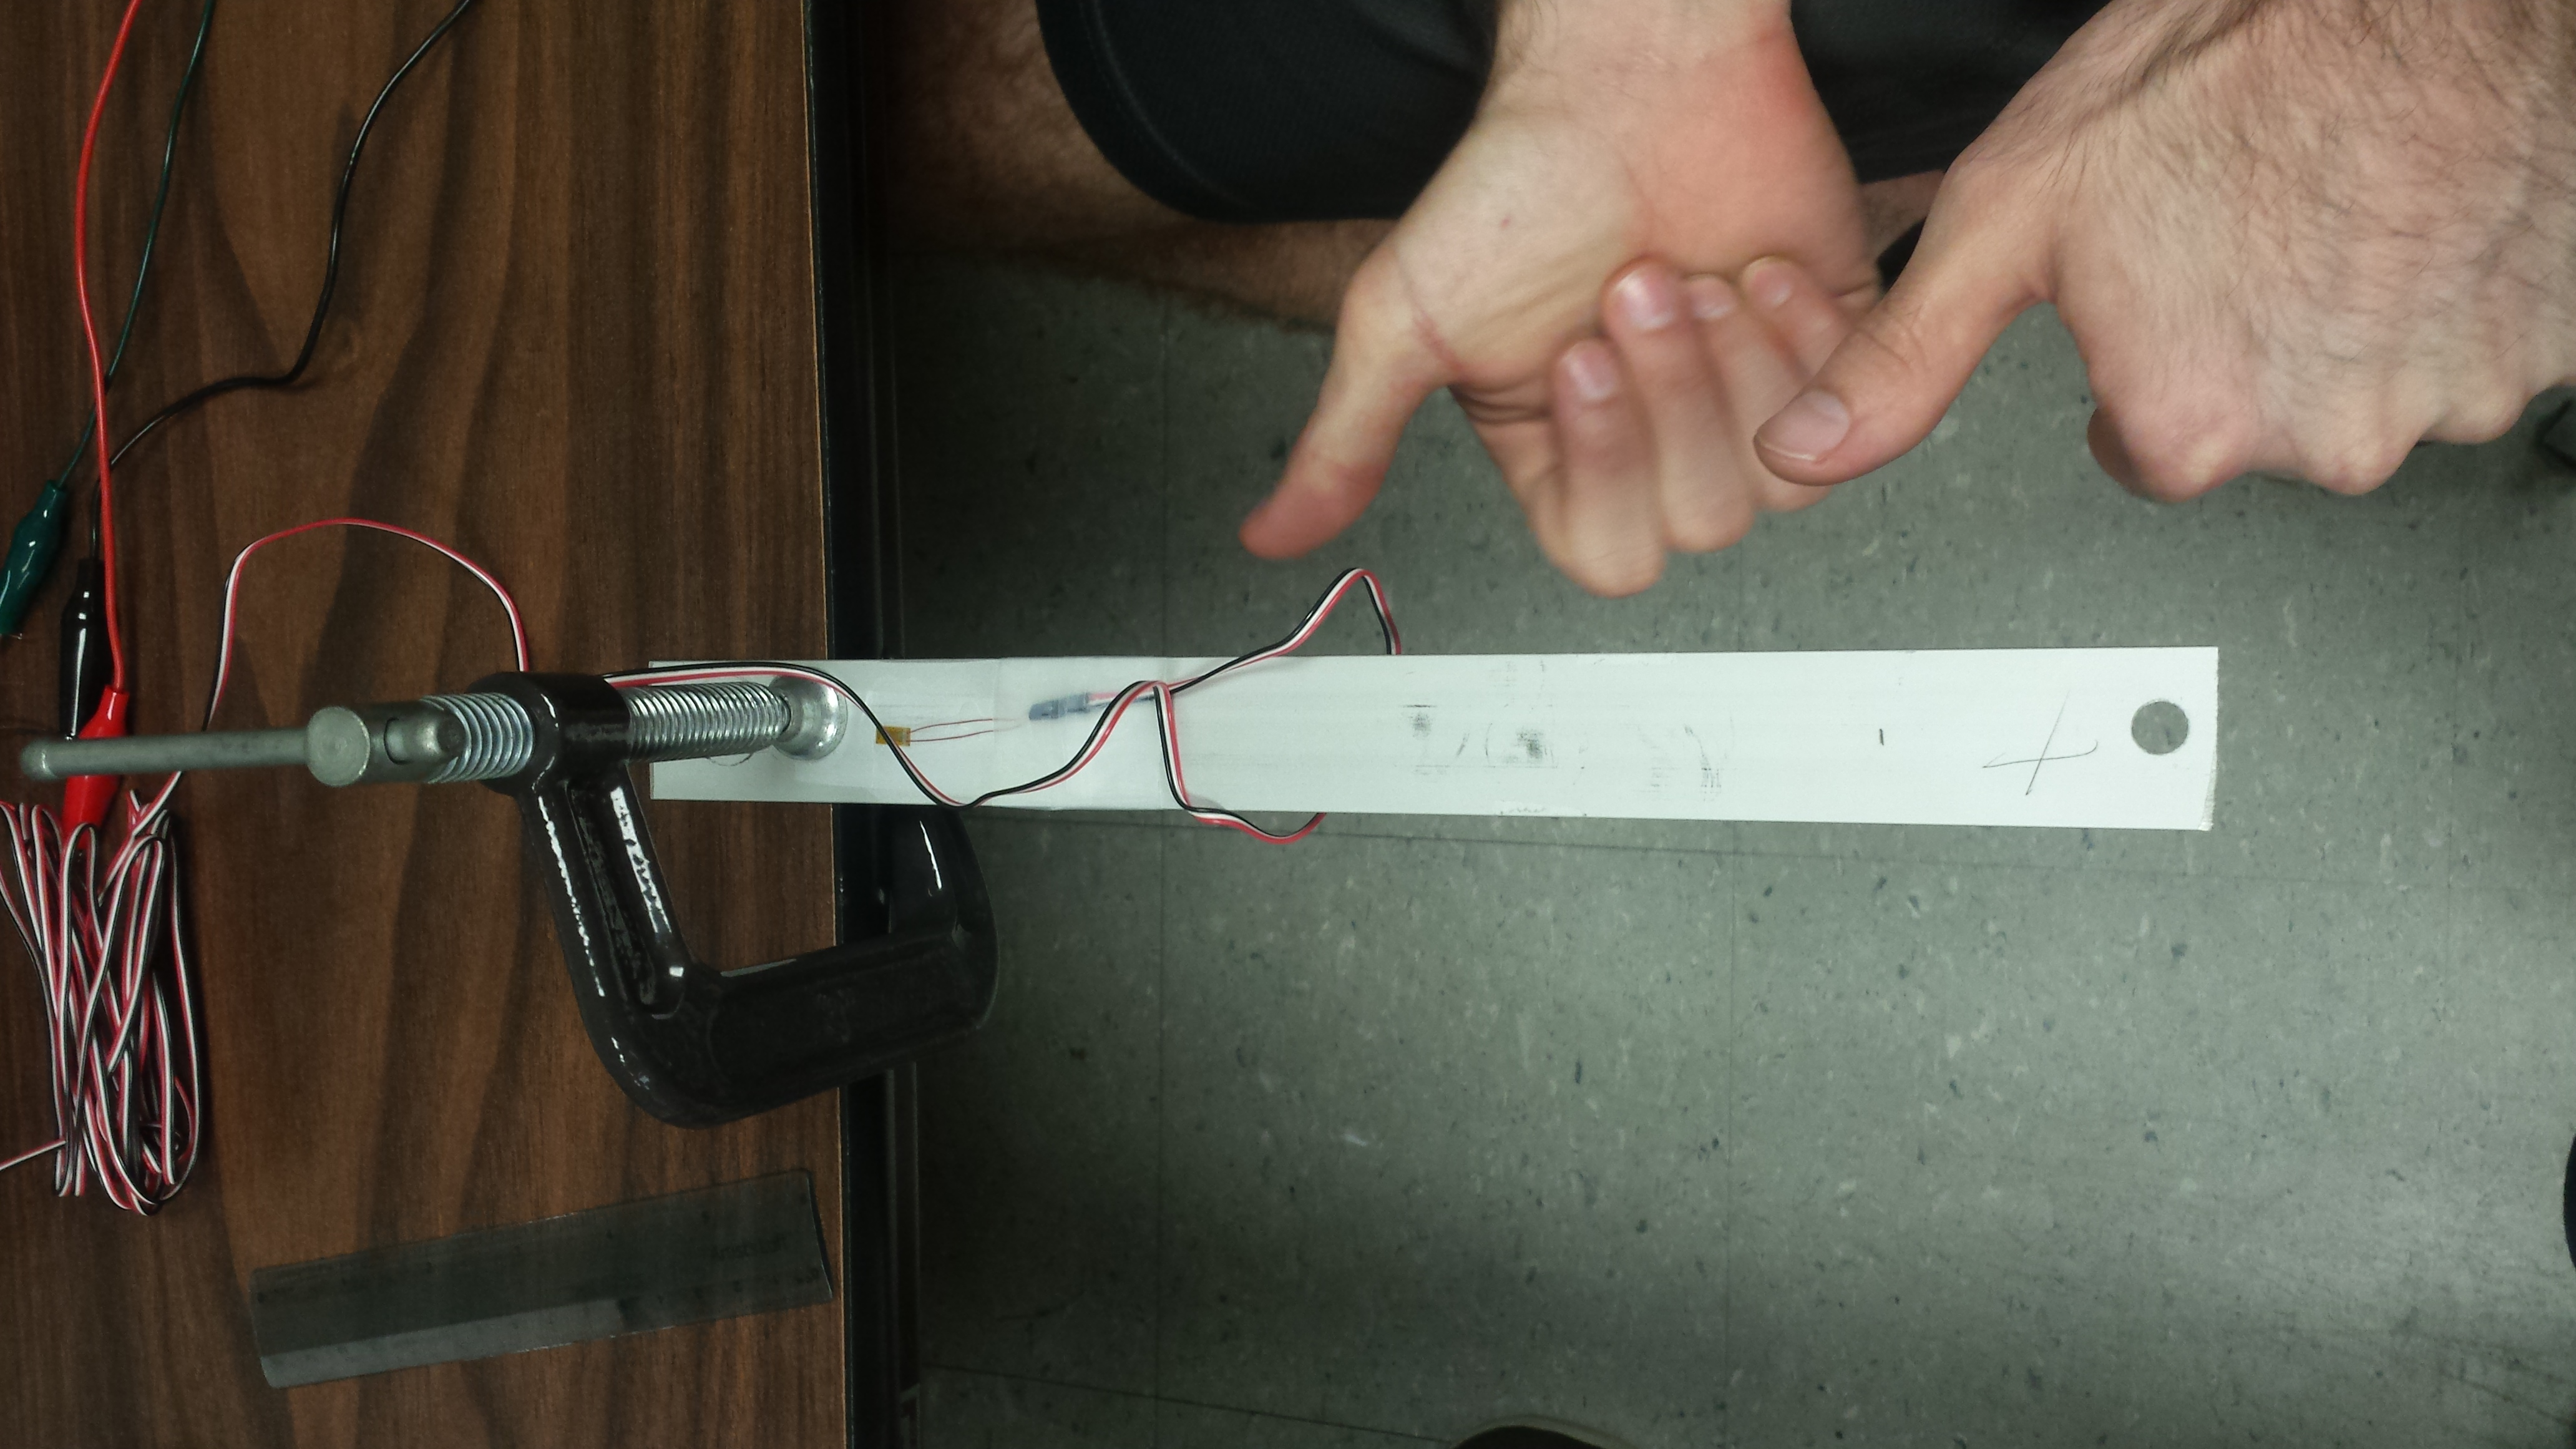
\includegraphics[width=3.8in, height=3.5in]{cantilever_beam.JPG}
    \caption{Cantilever Beam}
\end{figure}

\newpage

% Figure 2
\begin{figure}[h!]  
  \centering
    \includegraphics[width=4in, height=4in]{simply_supported_beam.JPG}
    \caption{Simply-Supported Beam}
\end{figure}

\bigskip


\section*{\fontsize{12}{12}\selectfont PROCEDURE}
The bending test was conducted in the metal forming lab on UL Lafayette campus. The only piece of equipment used, besides the beams and weights, was a magnetic dial indicator capable of returning readings in thousandths of an inch. The configuration shown in Figure 1 resembles the setup for the cantilever beam. The weight hanging from the cantilever beam was 1.09 kg, and measurements for deflections were recorded every half inch from the support, for a total of 15.5 inches. The configuration in Figure 2 resembles the setup for both of the simply-supported beams. The weight hanging from the simply-supported beams was 0.545 kg, and the deflections were also recorded every half inch starting at the support, for a total of 8 inches.
\bigskip

Along with measured deflections, theoretical deflections were also calculated using (5) and (6). The measured and calculated deflections were both plotted as a function of distance from the beam support on the same plot for each beam. The bending stress for each beam was also calculated and plotted as a function of distance from the support. 
\bigskip


\bigskip
\bigskip  

\newpage


\section*{\fontsize{12}{12}\selectfont RESLTS AND DISCUSSION}
The data recorded and calculated from the cantilever, aluminum simply-supported, and steel simply-supported experiments are shown in Tables 1, 2, and 3 respectively. A plot of the calculated and experimental cantilever beam deflections are shown in Figure 3. It can be seen that the experimental data closely matches the calculated data. The data also shows that the beam tends to deflect more as the distance from the beam support is increased.
\bigskip
\bigskip

% table1
\begin{center}
Table 1
\\
\emph{Cantilever Beam Data}
\\
\bigskip
\begin{tabular}{ccccc}
\hline
\begin{tabular}[c]{@{}c@{}}Distance\\ (mm)\end{tabular} & \begin{tabular}[c]{@{}c@{}}Measured Deflection\\ (mm)\end{tabular} & \begin{tabular}[c]{@{}c@{}}Calculated Deflection\\ (mm)\end{tabular} & \begin{tabular}[c]{@{}c@{}}Bending Moment\\ (N-m)\end{tabular} & \begin{tabular}[c]{@{}c@{}}Bending Stress\\ (MPa)\end{tabular} \\
\hline
0                    & -0.0191              & 0                    & -4.0740              & 11.4723              \\
12.7                 & -0.0381              & -0.0013              & -3.9382              & 11.0899              \\
25.4                 & -0.0508              & -0.0053              & -3.8024              & 10.7075              \\
38.1                 & -0.0762              & -0.0118              & -3.6666              & 10.3251              \\
50.8                 & -0.0762              & -0.0207              & -3.5308              & 9.9427               \\
63.5                 & -0.1016              & -0.0320              & -3.3950              & 9.5603               \\
76.2                 & -0.1270              & -0.0455              & -3.2592              & 9.1779               \\
88.9                 & -0.1270              & -0.0612              & -3.1234              & 8.7954               \\
101.6                & -0.1524              & -0.0790              & -2.9876              & 8.4130               \\
114.3                & -0.1778              & -0.0988              & -2.8518              & 8.0306               \\
127.0                & -0.2159              & -0.1204              & -2.7160              & 7.6482               \\
139.7                & -0.2286              & -0.1439              & -2.5802              & 7.2658               \\
152.4                & -0.2540              & -0.1691              & -2.4444              & 6.8834               \\
165.1                & -0.2794              & -0.1959              & -2.3086              & 6.5010               \\
177.8                & -0.2921              & -0.2242              & -2.1728              & 6.1186               \\
190.5                & -0.3048              & -0.2540              & -2.0370              & 5.7362               \\
203.2                & -0.3302              & -0.2852              & -1.9012              & 5.3538               \\
215.9                & -0.3556              & -0.3176              & -1.7654              & 4.9713               \\
228.6                & -0.4064              & -0.3511              & -1.6296              & 4.5889               \\
241.3                & -0.4318              & -0.3858              & -1.4938              & 4.2065               \\
254.0                & -0.4572              & -0.4215              & -1.3580              & 3.8241               \\
266.7                & -0.5080              & -0.4580              & -1.2222              & 3.4417               \\
279.4                & -0.5080              & -0.4954              & -1.0864              & 3.0593               \\
292.1                & -0.5334              & -0.5335              & -0.9506              & 2.6769               \\
304.8                & -0.5842              & -0.5722              & -0.8148              & 2.2945               \\
317.5                & -0.6096              & -0.6115              & -0.6790              & 1.9121               \\
330.2                & -0.6096              & -0.6512              & -0.5432              & 1.5296               \\
342.9                & -0.6604              & -0.6913              & -0.4074              & 1.1472               \\
355.6                & -0.6858              & -0.7317              & -0.2716              & 0.7648               \\
368.3                & -0.7366              & -0.7722              & -0.1358              & 0.3824               \\
381.0                & -0.7874              & -0.8128              & 0                    & 0                    \\
\hline
\multicolumn{1}{l}{} & \multicolumn{1}{l}{} & \multicolumn{1}{l}{} & \multicolumn{1}{l}{} & \multicolumn{1}{l}{}
\end{tabular}
\end{center}
% \end{table}

\newpage

% table2
\begin{center}
Table 2
\\
\emph{Simply-Supported Beam (Aluminum) Data}
\\
\bigskip
\begin{tabular}{ccccc}
\hline
\begin{tabular}[c]{@{}c@{}}Distance\\ (mm)\end{tabular} & \begin{tabular}[c]{@{}c@{}}Measured Deflection\\ (mm)\end{tabular} & \begin{tabular}[c]{@{}c@{}}Calculated Deflection\\ (mm)\end{tabular} & \begin{tabular}[c]{@{}c@{}}Bending Moment\\ (N-m)\end{tabular} & \begin{tabular}[c]{@{}c@{}}Bending Stress\\ (MPa)\end{tabular} \\
\hline
0     & 0       & 0       & 0      & 0      \\
12.7  & -0.0889 & -0.0923 & 0.0339 & 0.5179 \\
25.4  & -0.1778 & -0.1840 & 0.0679 & 1.0359 \\
38.1  & -0.2540 & -0.2741 & 0.1018 & 1.5538 \\
50.8  & -0.3429 & -0.3621 & 0.1358 & 2.0718 \\
63.5  & -0.4064 & -0.4473 & 0.1697 & 2.5897 \\
76.2  & -0.4826 & -0.5288 & 0.2037 & 3.1076 \\
88.9  & -0.5334 & -0.6059 & 0.2376 & 3.6256 \\
101.6 & -0.6223 & -0.6781 & 0.2716 & 4.1435 \\
114.3 & -0.7112 & -0.7444 & 0.3055 & 4.6615 \\
127.0 & -0.7366 & -0.8042 & 0.3395 & 5.1794 \\
139.7 & -0.8128 & -0.8569 & 0.3734 & 5.6973 \\
152.4 & -0.8255 & -0.9015 & 0.4074 & 6.2153 \\
165.1 & -0.8636 & -0.9375 & 0.4413 & 6.7332 \\
177.8 & -0.9144 & -0.9641 & 0.4753 & 7.2512 \\
190.5 & -0.9271 & -0.9806 & 0.5092 & 7.7691 \\
203.2 & -0.9652 & -0.9863 & 0.5432 & 8.2870 \\
\hline
\end{tabular}
\end{center}

\bigskip
\bigskip

% table3
\begin{center}
Table 3 
\\
\emph{Simply-Supported Beam (Steel) Data}
\\
\bigskip
\begin{tabular}{ccccc}
\hline
\begin{tabular}[c]{@{}c@{}}Distance\\ (mm)\end{tabular} & \begin{tabular}[c]{@{}c@{}}Measured Deflection\\ (mm)\end{tabular} & \begin{tabular}[c]{@{}c@{}}Calculated Deflection\\ (mm)\end{tabular} & \begin{tabular}[c]{@{}c@{}}Bending Moment\\ (N-m)\end{tabular} & \begin{tabular}[c]{@{}c@{}}Bending Stress\\ (MPa)\end{tabular} \\
\hline
0     & 0       & 0       & 0      & 0      \\
12.7  & -0.0127 & -0.0375 & 0.0339 & 0.5736 \\
25.4  & -0.0508 & -0.0747 & 0.0679 & 1.1472 \\
38.1  & -0.0762 & -0.1113 & 0.1018 & 1.7207 \\
50.8  & -0.1016 & -0.1470 & 0.1358 & 2.2943 \\
63.5  & -0.1524 & -0.1816 & 0.1697 & 2.8679 \\
76.2  & -0.1778 & -0.2147 & 0.2037 & 3.4415 \\
88.9  & -0.2032 & -0.2460 & 0.2376 & 4.0150 \\
101.6 & -0.2286 & -0.2753 & 0.2716 & 4.5886 \\
114.3 & -0.2794 & -0.3022 & 0.3055 & 5.1622 \\
127.0 & -0.2921 & -0.3265 & 0.3395 & 5.7358 \\
139.7 & -0.3048 & -0.3478 & 0.3734 & 6.3093 \\
152.4 & -0.3429 & -0.3660 & 0.4074 & 6.8829 \\
165.1 & -0.3683 & -0.3806 & 0.4413 & 7.4565 \\
177.8 & -0.3683 & -0.3914 & 0.4753 & 8.0301 \\
190.5 & -0.3810 & -0.3981 & 0.5092 & 8.6036 \\
203.2 & -0.3937 & -0.4004 & 0.5432 & 9.1772 \\
\hline
\end{tabular}
\end{center}

\newpage

% Figure 3
\begin{figure}[h!]  
  \centering
    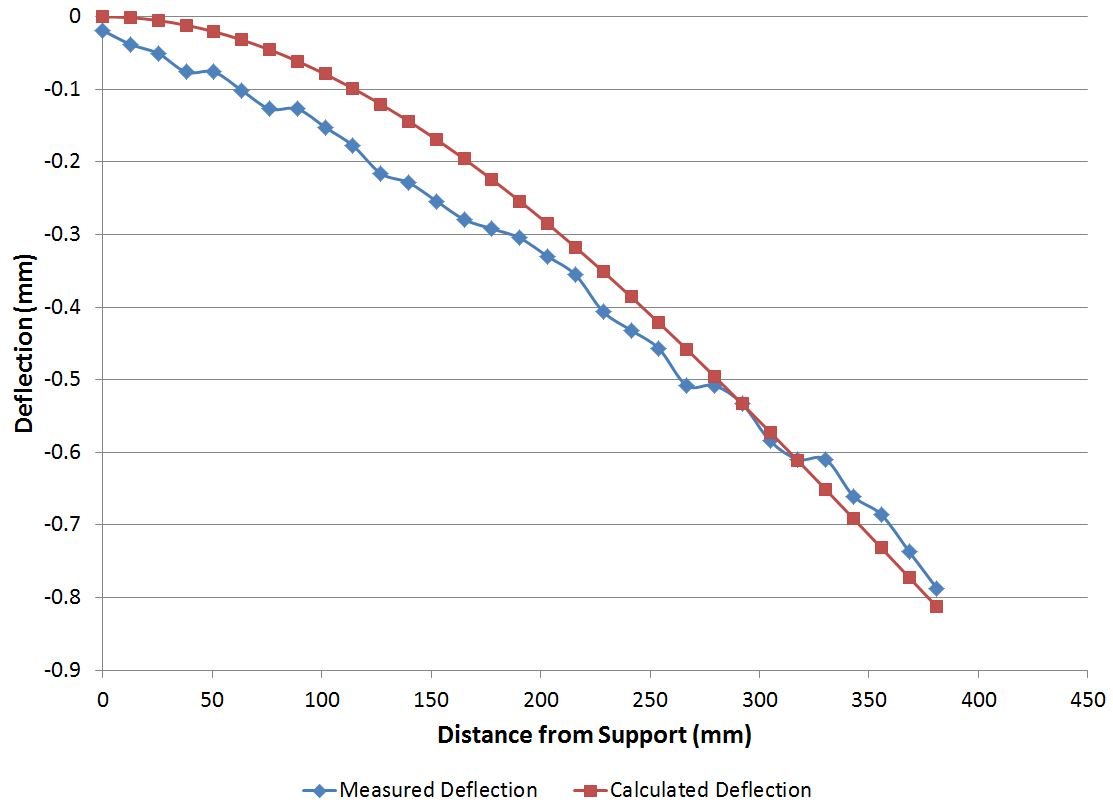
\includegraphics[width=\linewidth,height=5in]{cantilever_deflection.JPG}
    \caption{Cantilever Beam Displacement}
\end{figure}
\bigskip
\bigskip

A plot of the aluminum simply-supported beam calculated and experimental deflections can be seen in Figure 4, and the same plot for the steel simply-supported beam is shown in Figure 5. As seen in both plots, the experimental data closely matches the calculated data. It can also be seen from both plots that for a simply-supported beam, the deflections closer to the middle of the beam are where max deflections occur. 
\bigskip

It should be noted, that unlike a cantilever beam, max deflections for a simply-supported beam occur when loaded at the middle of the beam rather than at the end. This is because the beam is supported at both ends, which would cancel any deflections occurring at the very ends of the beam. It should also be noted when comparing the two plots, that the steel deflects less than the aluminum beam, since steel is a stronger material and therefore has a higher modulus of elasticity. 
\bigskip

\newpage

% Figure 4
\begin{figure}[h!]  
  \centering
    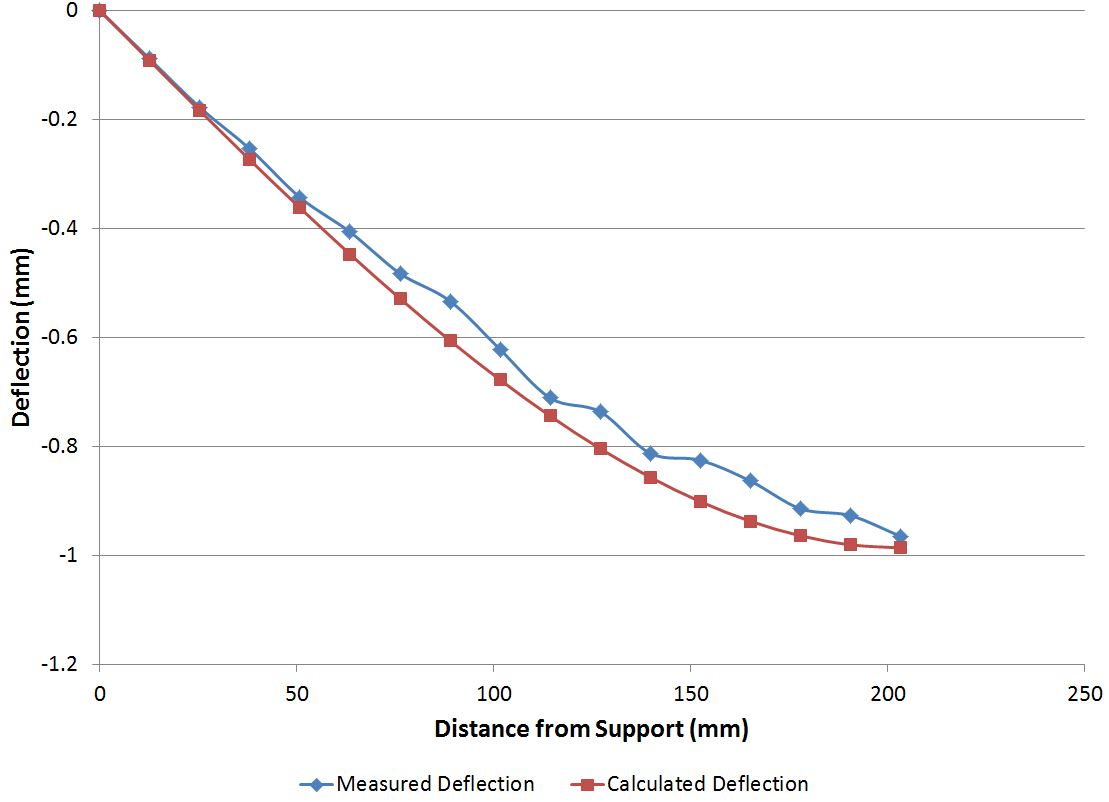
\includegraphics[width=\linewidth,height=3.8in]{simp_support_a_deflection.JPG}
    \caption{Simply-Supported Beam Deflections (Aluminum)}
\end{figure}

\bigskip

% Figure 5
\begin{figure}[h!]  
  \centering
    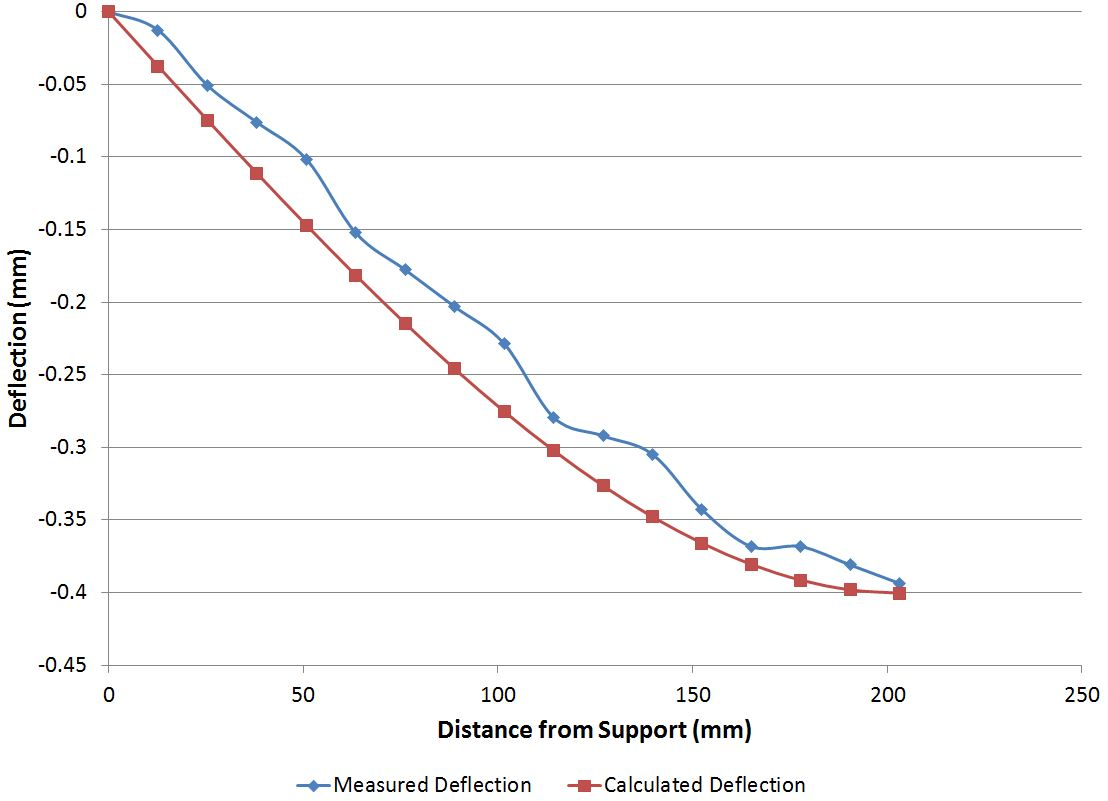
\includegraphics[width=\linewidth,height=3.8in]{simp_support_s_deflection.JPG}
    \caption{Simply-Supported Beam Deflections (Steel)}
\end{figure}


\newpage

Notice that the deflection plots for all three beams tend to follow a quadratic trend. This is because the equations for deflections of both types of beams are quadratic functions of distance from the beam support, as seen in (5) and (6).
\bigskip  

The max bending stress at each measured interval is also plotted for each beam. The plots for bending stress versus distance from the beam support can be seen in Figures 6, 7, and 8. It should be noted that the bending stress decreases further from the support for a cantilever beam, while in the case of a simply-supported beam, it rises. This is because for a cantilever beam, the bending moment is higher close to the support, while the bending moment in a simply-supported beam is higher close to the load. As seen in (4), bending stress is directly dependent on the bending moment.
\bigskip

Also, notice that all three plots follow a linear behavior. This is because the bending moments for both types of beams are linear functions of distance \emph{x}, as seen before in (2) and (3). These equations are linear because the loadings in this experiment are concentrated loads. According to [2], if the loading on the beam were a distributed load, the equation would be a \emph{quadratic} function of distance from the beam support rather than linear.
\bigskip
\bigskip
\bigskip


% Figure 6
\begin{figure}[h!]  
  \centering
    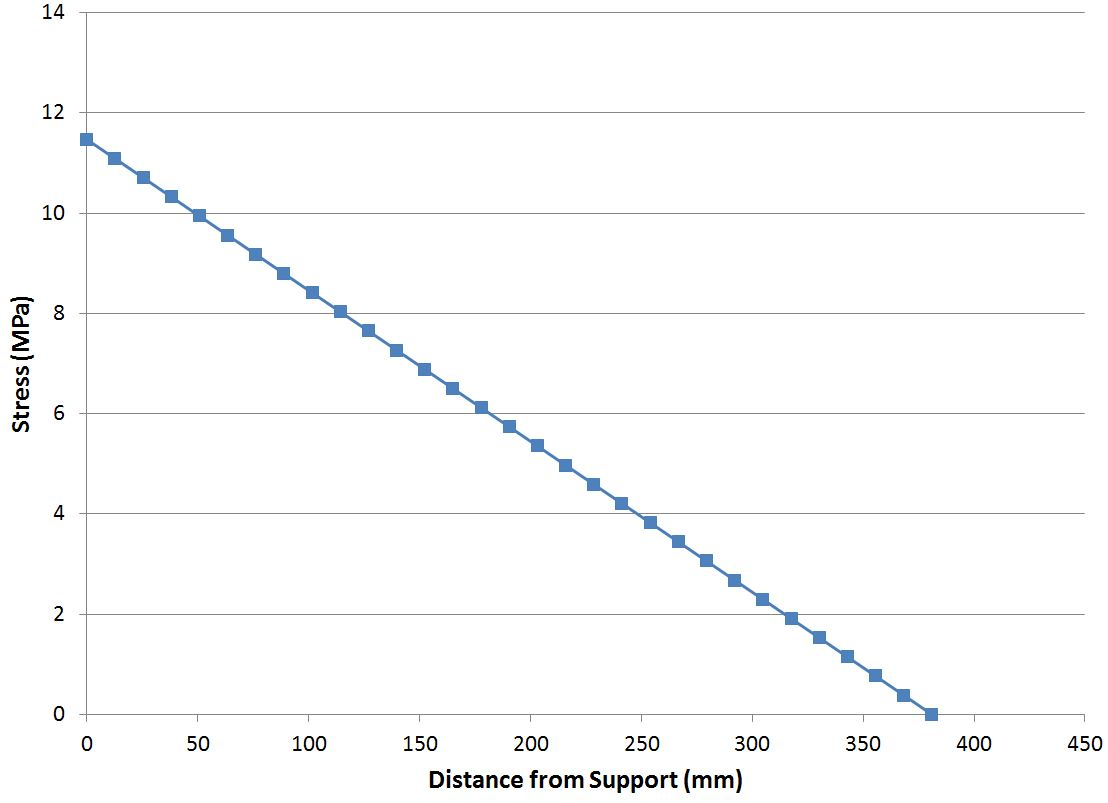
\includegraphics[width=\linewidth, height=4.5in]{cantilever_stress_vs_distance.JPG}
    \caption{Cantilever Beam Bending Stress} 
\end{figure}


\newpage


% Figure 7
\begin{figure}[h!]  
  \centering
    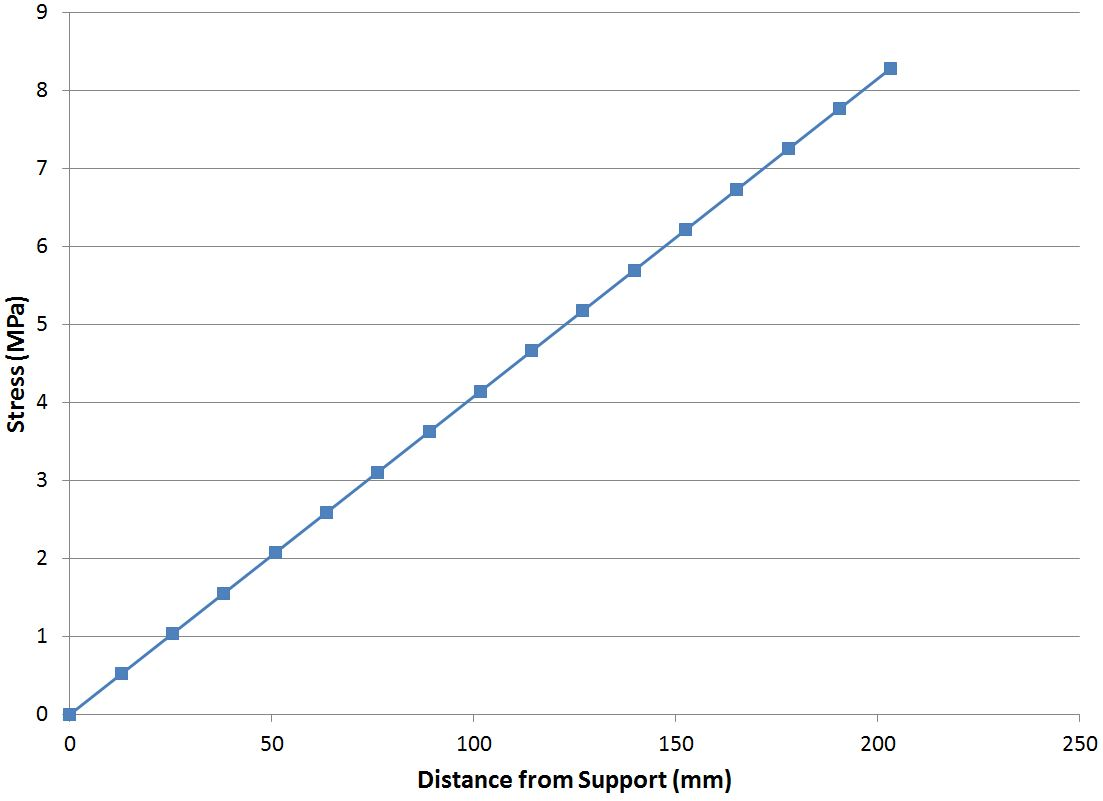
\includegraphics[width=\linewidth, height=3.8in]{simp_support_a_stress_vs_distance.JPG}
    \caption{Simply-Supported Beam Bending Stress (Aluminum)} 
\end{figure}

\bigskip

% Figure 8
\begin{figure}[h!]  
  \centering
    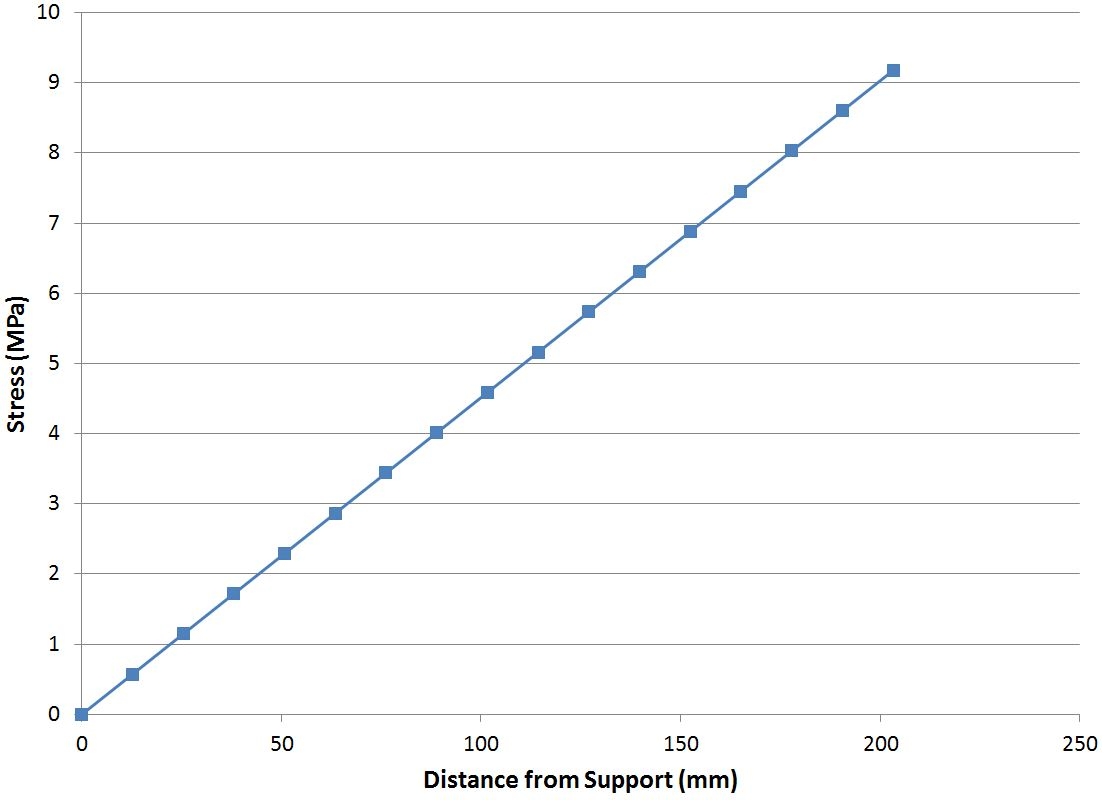
\includegraphics[width=\linewidth, height=3.8in]{simp_support_s_stress_vs_distance.JPG}
    \caption{Simply-Supported Beam Bending Stress (Steel)} 
\end{figure}


\newpage

The design factor for any product is given by (7). For each beam, the design factor was calculated for each calculated bending stress, excluding zero which results in a design factor of infinity. The yield stress for AISI 1006 HRS steel is 170 MPa, and the yield stress for 2014 aluminum is 76 MPa. The design factors for the cantilever, aluminum simply-supported, and steel simply-supported beams are shown in Figures 9, 10, and 11 respectively. Generally, a high design factor will yield a durable, safe design. A factor too high will result in an over-engineered product which will waste cost and material in manufacturing, and possibly even a product which is too cumbersome for the product.
\bigskip


% Equation 7
\begin{equation}
n=\frac{\sigma_{yield}}{\sigma_{calculated}}
\end{equation}
\bigskip
\bigskip



% Figure 9
\begin{figure}[h!]  
  \centering
    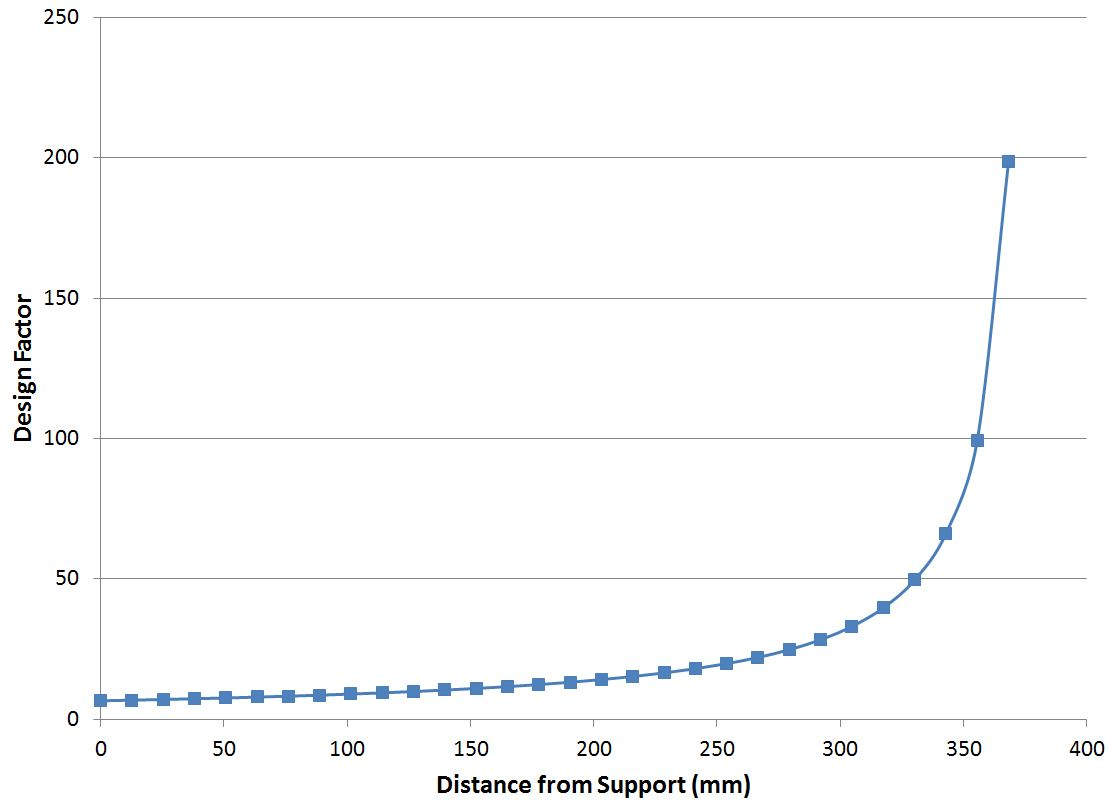
\includegraphics[width=\linewidth]{cantilever_df.JPG}
    \caption{Cantilever Beam Design Factor} 
\end{figure}

\newpage

% Figure 10
\begin{figure}[h!]  
  \centering
    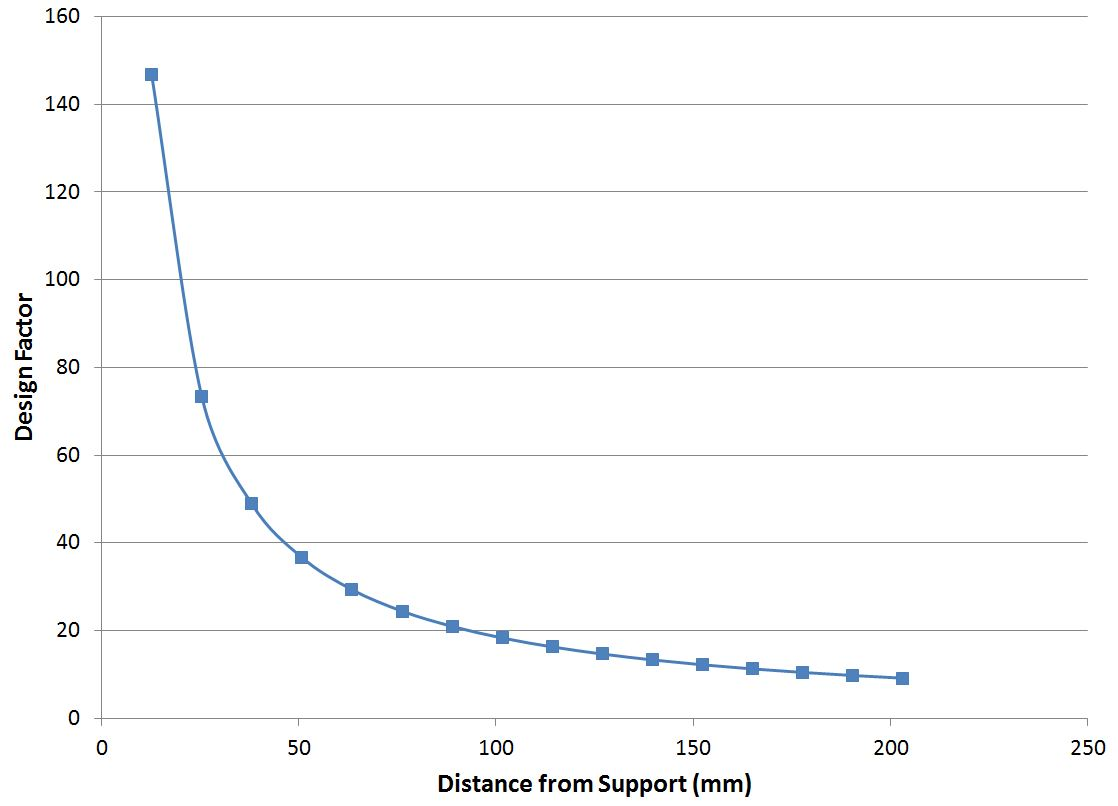
\includegraphics[width=\linewidth, height=3.8in]{ss_a_df.JPG}
    \caption{Simply-Supported Beam Design Factor (Aluminum)} 
\end{figure}

\bigskip

% Figure 11
\begin{figure}[h!]  
  \centering
    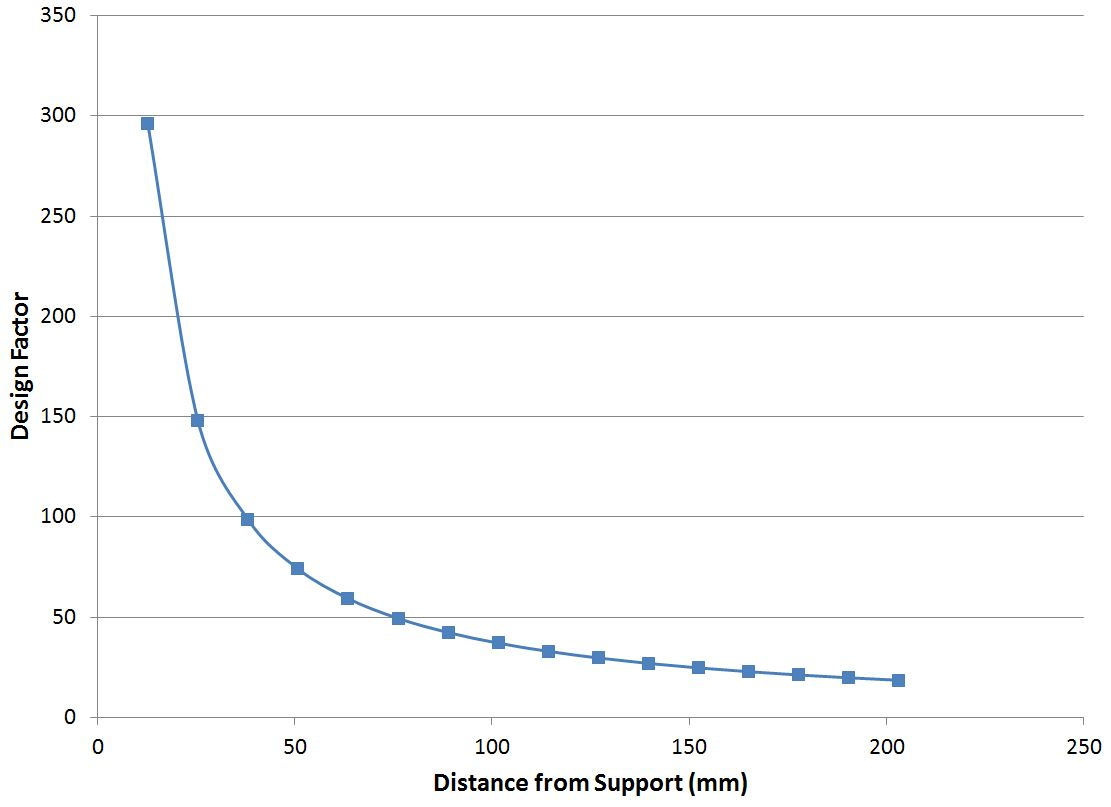
\includegraphics[width=\linewidth, height=3.8in]{ss_s_df.JPG}
    \caption{Simply-Supported Beam Design Factor (Steel)} 
\end{figure}

\newpage


\section*{\fontsize{12}{12}\selectfont CONCLUSION}
The data from this beam bending test, performed on UL campus, has been analyzed and plotted. The originally recorded data was also used to calculate the deflections, as well as the bending stress, for each beam. The results calculated from the data closely matched the data measured in the experiment. 
\bigskip

The data also shows that cantilever beams deflect most towards the end of the beam when loaded as shown in Figure 1, while simply-supported beams deflect most towards the middle of the beam when loaded as shown in Figure 2. It was seen that the deflections of both types of beams followed a quadratic trend, just as (5) and (6) would suggest.
\bigskip

It was also shown that the bending stress for cantilever beams is highest near the beam support, while the bending stress for simply-supported beams is highest near the loading. This difference is caused by the fact that the beam is supported on both ends in a simply-supported beam, which restricts the movement of the beam at both ends. This causes the bending stress to reach a maximum at the point furthest from both supports in the case of this experiment, which is the middle of the beam. Also, the moments for both types of beams follows a linear trend, just as (2) and (3) would suggest. This causes the bending stress to also be linear because it is directly dependent on the bending moment.
\bigskip

It has been concluded that the behavior of the beams in the experiment closely match the theoretical behavior of the materials. This confirms that the method of analysis by equations (1)-(6) is accurate enough for use in practice as long as the beams are only exposed to concentrated loads. If the beams in an application are exposed to more sophisticated loads, such as distributed loads, then these equations will need to be re-derived for the application. Also, the design factor should be utilized in designing any member of a mechanism, and should be chosen to optimize the design for a balance between safety and practicality.
\bigskip


\section*{\fontsize{12}{12}\selectfont REFERENCES}

\begin{thebibliography}{2}

\bibitem{}
Hibbeler, R.C., 2014, \emph{Mechanics of Materials}, Prentice Hall, Upper Saddle River, NJ, Chap. 6.

\bibitem{}
“Shear Forces and Bending Moments,” \emph{Open Course Ware (National Tsing Hua University)}, n.d., from
\\http://ocw.nthu.edu.tw/ocw/upload/8/253/Chapter\_4-98.pdf


\end{thebibliography}

%\section*{\fontsize{12}{12}\selectfont APPENDIX}

%\begin{table}[h!]
%  \caption{}
%  \includegraphics[width=\linewidth]{table1.png}
%\end{table}

\end{document}
----------------------------%TEmplates-------------------------------

-------------------------Figure-----------------------

\begin{figure}[h!]  
  \centering
    \includegraphics[width=\linewidth]{**file**}
    \caption{Docking Station}
\end{figure}

---------------------------Table-----------------------
\begin{table}[ht]
\caption{Nonlinear Model Results} % title of Table
\centering % used for centering table
\begin{tabular}{c c c c} % centered columns (4 columns)
\hline\hline %inserts double horizontal lines
Case & Method\#1 & Method\#2 & Method\#3 \\ [0.5ex] % inserts table
%heading
\hline % inserts single horizontal line
1 & 50 & 837 & 970 \\ % inserting body of the table
2 & 47 & 877 & 230 \\
3 & 31 & 25 & 415 \\
4 & 35 & 144 & 2356 \\
5 & 45 & 300 & 556 \\ [1ex] % [1ex] adds vertical space
\hline %inserts single line
\end{tabular}
\label{table:nonlin} % is used to refer this table in the text
\end{table}



probably best to insert as an image from excel

\bigskip\\
\begin{table}[h!]
  \caption{}
  \includegraphics[width=\linewidth]{**file**}
\end{table}
\bigskip\\





-----------------------------Equations------------------------
-----------------------------Regular
\begin{equation}
a = b + c
\end{equation}

--------------------------------- Multiline
\begin{multline}
a = b + c + d + e + f
+ g + h + i + j \\
+ k + l + m + n + o
\end{multline}

-------------------------------Citations-------------------------
\bibitem{Author last name}
  Last, First., year of publication,
  article name, book(etc) name, from \\
  link goes here

----------------------------------other-----------------------------

equations:
http://moser-isi.ethz.ch/docs/typeset_equations.pdf

citations:
http://library.missouri.edu/engineering/about/guides/asme
https://www.asme.org/shop/proceedings/conference-publications/references